\chapter{Data Preparation e Data Cleaning}
\label{ch:data-preparation}

\begin{noteblock}{Laboratorio Pratico: Esecuzione Interattiva su Jupyter Notebook}
I codici Python presentati in questo capitolo corrispondono al notebook di laboratorio:
\begin{itemize}
    \item \textbf{Notebook:} \href{http://localhost:8888/lab/tree/notebooks/2_feature_engineering_and_data_representation.ipynb}{\texttt{2\_feature\_engineering\_\dots.ipynb}}
    \item \textbf{Accesso diretto:} \href{http://localhost:8888/lab/tree/notebooks/2_feature_engineering_and_data_representation.ipynb}{\textbf{[Apri su Jupyter Lab]}} \quad (\url{http://localhost:8888})
    \item \textbf{Avvio rapido del container:} Da terminale nella radice del progetto: \texttt{docker compose up jupyter}
    \item \textbf{Cartella di lavoro locale:} \texttt{Data-Mining/notebooks/} (dataset posizionati in \texttt{./data\_notebook/}).
\end{itemize}
\end{noteblock}

\FloatBarrier
\section{Obiettivi della Data Preparation}

Se la fase di \textit{Data Understanding} (Capitolo~\ref{ch:data-understanding}) risponde alla domanda fondamentale \textit{<<come sono fatti i dati e quali criticità presentano?>>}, la fase di \textbf{Data Preparation} (\textit{Preparazione dei Dati}) traduce tali evidenze analitiche in azioni trasformative concrete:
\begin{center}
\resizebox{0.92\linewidth}{!}{%
\begin{tikzpicture}[
    box/.style={rectangle, rounded corners=6pt, draw=blue!70, fill=blue!4, thick, inner sep=10pt, text width=5.6cm, minimum height=3.6cm, align=left},
    arrow/.style={-Stealth, very thick, color=blue!75}
]
    \node[box] (du) at (0, 0) {
        \centering\textbf{\large Data Understanding}\\[8pt]
        \raggedright\small
        $\bullet$~Rilevamento valori mancanti\\
        $\bullet$~Rilevamento di outlier\\
        $\bullet$~Studio delle distribuzioni\\
        $\bullet$~Analisi correlazioni e legami
    };
    \node[box] (dp) at (10.5, 0) {
        \centering\textbf{\large Data Preparation}\\[8pt]
        \raggedright\small
        $\bullet$~Selezione feature e istanze\\
        $\bullet$~Riduzione di dimensionalit\`a\\
        $\bullet$~Imputazione e pulizia anomalie\\
        $\bullet$~Trasformazione e codifica
    };
    
    \draw[arrow] (du.east) -- node[above=3pt, font=\scriptsize\bfseries, text=blue!90!black, fill=white, inner sep=3pt, rounded corners=3pt, draw=blue!30] {Guida le decisioni} (dp.west);
\end{tikzpicture}%
}
\end{center}

Gli obiettivi primari della preparazione dei dati si riassumono in:
\begin{itemize}
    \item \textbf{Miglioramento della qualità dei dati (\textit{Data Quality}):} Eliminare o correggere rumore, inconsistenze sintattiche e semantiche.
    \item \textbf{Adattamento ai requisiti degli algoritmi:} Molti algoritmi di Data Mining e Machine Learning richiedono formati specifici (ad esempio variabili binarie asimmetriche per le regole associative, oppure feature con scala numerica omogenea per metodi basati sulla distanza euclidea).
    \item \textbf{Efficienza computazionale e contrasto della dimensionalità:} Ridurre la complessità spaziale e temporale mediante campionamento (\textit{data reduction}) o selezione/proiezione di attributi (\textit{dimensionality reduction}).
\end{itemize}

Le macro-tecniche di Data Preparation comprendono:
\begin{enumerate}
    \item \textbf{Aggregazione (\textit{Aggregation}):} Combinazione di oggetti o attributi su scale più ampie.
    \item \textbf{Riduzione dei Dati tramite Campionamento (\textit{Sampling}):} Selezione di un sottoinsieme rappresentativo di istanze.
    \item \textbf{Riduzione di Dimensionalità (\textit{Dimensionality Reduction}):} Selezione o estrazione/proiezione (PCA, SVD).
    \item \textbf{Creazione di Nuove Feature (\textit{Feature Creation}):} Feature construction guidata dal dominio.
    \item \textbf{Discretizzazione e Binarizzazione:} Conversione continuo-discreto e encoding categorico.
    \item \textbf{Trasformazione degli Attributi (\textit{Attribute Transformation}):} Normalizzazione, scalatura decimale, trasformazioni logaritmiche e stabilizzazione della varianza.
\end{enumerate}

---

\section{Aggregazione dei Dati}

\begin{definition}[Aggregazione]
L'\textbf{aggregazione} consiste nella combinazione di due o più attributi (o di due o più oggetti/record) in un singolo attributo (o singolo oggetto aggregato).
\end{definition}

L'aggregazione persegue tre scopi metodologici fondamentali:
\begin{itemize}
    \item \textbf{Riduzione della dimensione dei dati:} Diminuisce drasticamente il numero di record (righe) o il numero di colonne (feature) da elaborare.
    \item \textbf{Cambiamento di scala temporale o spaziale:}
    \begin{itemize}
        \item \textit{Aggregazione spaziale:} Misurazioni registrate per singola città o quartiere aggregate a livello regionale o nazionale.
        \item \textit{Aggregazione temporale:} Transazioni orarie o giornaliere aggregate su base settimanale, mensile o annuale.
    \end{itemize}
    \item \textbf{Stabilizzazione statistica del dato:} I dati aggregati presentano intrinsecamente \textbf{minore variabilità} rispetto alle misurazioni individuali a granularità fine.
\end{itemize}

\subsection{Esempio: Precipitazioni in Australia (1982--1993)}
Si consideri lo studio delle precipitazioni su centinaia di stazioni meteorologiche terrestri in Australia per il periodo 1982--1993:
\begin{itemize}
    \item Confrontando la deviazione standard delle precipitazioni medie \textbf{mensili} rispetto a quella delle precipitazioni medie \textbf{annuali}, si osserva che la deviazione standard annuale è fortemente concentrata su valori vicini allo zero (Figura~\ref{fig:precipitation-aggregation}).
    \item L'aggregazione temporale annuale comprime i picchi transitori e rimuove la dispersione stagionale. Tuttavia, se l'obiettivo di data mining è studiare \textbf{i pattern climatici stagionali o monsonici}, l'istogramma mensile risulta di gran lunga più informativo e appropriato rispetto a quello annuale.
\end{itemize}

\begin{figure}[H]
\centering

\includegraphics[width=0.94\textwidth]{precipitation_aggregation.pdf}
\caption{Effetto dell'aggregazione sulla dispersione statistica (Esempio Precipitazioni in Australia): a sinistra la deviazione standard delle medie mensili (mostra ampia variabilità stagionale); a destra la deviazione standard delle medie annuali (evidenzia come l'aggregazione comprima la varianza e stabilizzi le osservazioni).}
\label{fig:precipitation-aggregation}
\end{figure}

---

\section{Riduzione dei Dati tramite Campionamento (Sampling)}

Il \textbf{campionamento} (\textit{Data Sampling}) rappresenta la tecnica cardine per la riduzione del numero di record (righe del dataset).

\begin{remark}[Principio Guida del Campionamento Efficace]
Un campione statistico $\mathcal{S}$ produce risultati analitici quasi identici a quelli ottenibili sull'intera popolazione $\mathcal{D}$ se e solo se $\mathcal{S}$ è \textbf{rappresentativo}.
Un campione è rappresentativo se possiede approssimativamente le stesse proprietà distributive di interesse del dataset originario.
\end{remark}

\subsection{Trade-off sulla Dimensione del Campione}
La scelta della cardinalità del campione riflette un compromesso analitico:
\begin{itemize}
    \item Un campione eccessivamente ridotto (es. 500 punti su 8000) perde la continuità geometrica dei pattern, disgrega i cluster densi e non consente di cogliere dettagli fini.
    \item Un campione sufficientemente dimensionato (es. 2000 punti) preserva la silhouette delle distribuzioni e le relazioni topologiche consentendo tempi di esecuzione notevolmente inferiori.
\end{itemize}

\begin{figure}[H]
\centering

\includegraphics[width=0.95\textwidth]{sampling_tradeoff.pdf}
\caption{Trade-off della dimensione del campione nel campionamento casuale: a sinistra la popolazione originaria ($N=8000$) con strutture non lineari complesse; al centro un sotto-campionamento eccessivo ($n=500$, $6.25\%$) che frammenta i cluster ed elimina dettagli; a destra un campione dimensionato efficacemente ($n=2000$, $25\%$) che preserva fedelmente la topologia e le densità con una netta riduzione del carico computazionale.}
\label{fig:sampling-tradeoff}
\end{figure}

\subsection{Tipologie di Campionamento}
Si distinguono due macro-famiglie di campionamento probabilistico:

\begin{enumerate}
    \item \textbf{Simple Random Sampling (Campionamento Casuale Semplice):} Ciascun oggetto della popolazione ha identica probabilità di estrazione:
    \begin{itemize}
        \item \textbf{Campionamento Senza Reintegro (\textit{Without Replacement}):} Una volta selezionato, l'oggetto viene rimosso dalla popolazione. Ciascun oggetto compare al più una sola volta nel campione.
        \item \textbf{Campionamento Con Reintegro (\textit{With Replacement}):} L'oggetto estratto non viene rimosso e può essere selezionato nuovamente. La popolazione rimane identica ad ogni estrazione.
    \end{itemize}
    \item \textbf{Campionamento Stratificato (\textit{Stratified Sampling}):} Si suddivide preliminarmente la popolazione in partizioni disgiunte (\textit{strati}), ciascuna caratterizzata da una modalità specifica di classe o da un cluster naturale di densità (Figura~\ref{fig:stratified-sampling-tikz}). Successivamente, si estraggono campioni casuali da ogni singolo strato in proporzione alla sua frequenza.
\end{enumerate}

\begin{figure}[H]
\centering
\resizebox{0.95\linewidth}{!}{%
\begin{tikzpicture}[
    box/.style={draw=gray!50, fill=gray!2, very thick, rounded corners=8pt},
    stratumA/.style={draw=blue!60, fill=blue!8, thick, rounded corners=6pt},
    stratumB/.style={draw=red!60, fill=red!8, thick, rounded corners=6pt},
    stratumC/.style={draw=teal!70, fill=teal!8, thick, rounded corners=6pt},
    ptA/.style={circle, fill=blue!80!black, draw=white, line width=0.5pt, inner sep=2.4pt},
    ptB/.style={circle, fill=red!80!black, draw=white, line width=0.5pt, inner sep=2.4pt},
    ptC/.style={circle, fill=teal!70!black, draw=white, line width=0.5pt, inner sep=2.4pt}
]
    % --- Pannello Sinistro: Dataset Originario ---
    \draw[box] (0, 0) rectangle (7.4, 4.8);
    \node[above=4pt, font=\bfseries\small, text=gray!90!black] at (3.7, 4.8) {Dataset Originario (Popolazione)};

    % Strato A (Blu)
    \draw[stratumA] (0.3, 2.6) rectangle (3.5, 4.4);
    \node[font=\scriptsize\bfseries, text=blue!80!black] at (1.9, 4.05) {Strato 1 (Blu)};
    \node[ptA] at (0.9, 3.3) {}; \node[ptA] at (1.5, 3.4) {}; \node[ptA] at (2.2, 3.3) {}; \node[ptA] at (2.9, 3.3) {};
    \node[ptA] at (1.2, 2.9) {}; \node[ptA] at (1.9, 2.9) {}; \node[ptA] at (2.6, 2.9) {};

    % Strato B (Rosso)
    \draw[stratumB] (3.9, 2.6) rectangle (7.1, 4.4);
    \node[font=\scriptsize\bfseries, text=red!80!black] at (5.5, 4.05) {Strato 2 (Rosso)};
    \node[ptB] at (4.5, 3.3) {}; \node[ptB] at (5.1, 3.4) {}; \node[ptB] at (5.8, 3.3) {}; \node[ptB] at (6.5, 3.3) {};
    \node[ptB] at (4.8, 2.9) {}; \node[ptB] at (5.5, 2.9) {}; \node[ptB] at (6.2, 2.9) {};

    % Strato C (Verde - Minoranza)
    \draw[stratumC] (1.6, 0.4) rectangle (5.8, 2.2);
    \node[font=\scriptsize\bfseries, text=teal!80!black] at (3.7, 1.85) {Strato 3 (Minoranza)};
    \node[ptC] at (2.6, 1.1) {}; \node[ptC] at (3.3, 1.3) {}; \node[ptC] at (4.0, 1.0) {}; \node[ptC] at (4.7, 1.2) {};

    % --- Frecce e Transizione Centrale ---
    \draw[-Stealth, line width=1.5pt, color=blue!75] (7.7, 2.4) -- (10.3, 2.4);
    \node[align=center, font=\scriptsize\bfseries, text=blue!90!black, fill=white, inner sep=3.5pt, rounded corners=3pt, draw=blue!30] at (9.0, 3.3) {Campionamento\\per Strato};
    \node[align=center, font=\scriptsize, text=gray!75!black] at (9.0, 1.4) {Quote di classe\\preservate};

    % --- Pannello Destro: Campione Stratificato ---
    \draw[box] (10.6, 0) rectangle (18.0, 4.8);
    \node[above=4pt, font=\bfseries\small, text=gray!90!black] at (14.3, 4.8) {Campione Stratificato Proporzionale};

    % Strato A Campionato
    \draw[stratumA] (10.9, 2.6) rectangle (14.1, 4.4);
    \node[font=\scriptsize\bfseries, text=blue!80!black] at (12.5, 4.05) {Strato 1};
    \node[ptA] at (11.8, 3.2) {}; \node[ptA] at (13.2, 3.2) {};

    % Strato B Campionato
    \draw[stratumB] (14.5, 2.6) rectangle (17.7, 4.4);
    \node[font=\scriptsize\bfseries, text=red!80!black] at (16.1, 4.05) {Strato 2};
    \node[ptB] at (15.4, 3.2) {}; \node[ptB] at (16.8, 3.2) {};

    % Strato C Campionato (Minoranza preservata!)
    \draw[stratumC] (12.1, 0.4) rectangle (16.5, 2.2);
    \node[font=\scriptsize\bfseries, text=teal!80!black] at (14.3, 1.85) {Strato 3 (Garantito!)};
    \node[ptC] at (14.3, 1.1) {};
\end{tikzpicture}%
}
\caption{Schema del Campionamento Stratificato: la popolazione viene partizionata in strati omogenei (classi o sottopopolazioni con picchi di densità); il campionamento casuale viene condotto separatamente all'interno di ogni strato, garantendo la presenza anche delle classi di minoranza.}
\label{fig:stratified-sampling-tikz}
\end{figure}

Il campionamento stratificato è indispensabile in presenza di \textbf{distribuzioni bimodali o con forti picchi di densità} e in contesti di \textbf{classi fortemente sbilanciate} (ad esempio rilevamento frodi, dove le transazioni fraudolente sono meno dell'1\% del totale).

---

\section{Riduzione di Dimensionalità}

Nei dataset multidimensionali moderni, gli oggetti sono descritti da centinaia o migliaia di attributi:
\begin{equation}
\mathbf{X} \in \mathbb{R}^{n \times p} \longrightarrow \mathbf{Z} \in \mathbb{R}^{n \times k} \quad \text{con } k \ll p
\end{equation}
In tale passaggio:
\begin{itemize}
    \item Gli oggetti (le $n$ righe) rimangono inalterati nella loro identità ontologica.
    \item Le coordinate cambiano: ogni osservazione riceve $k$ nuove coordinate sintetiche.
    \item La struttura geometrica sottostante viene selezionata in funzione della relazione da preservare (ad esempio la varianza globale o la separazione tra classi).
\end{itemize}

\subsection{La Maledizione della Dimensionalità (\textit{Curse of Dimensionality})}
All'aumentare del numero di dimensioni $p$, il volume dello spazio vettoriale cresce esponenzialmente rispetto al numero finito di osservazioni campionate $n$:
\begin{itemize}
    \item \textbf{Iper-spazio vuoto (\textit{Data Sparsity}):} I punti campionati diventano straordinariamente isolati nel volume dell'ipercubo unitario $[0, 1]^p$. Per preservare una densità campionaria costante al crescere delle dimensioni, la dimensione del campione $n$ dovrebbe crescere esponenzialmente con $p$, condizione irrealizzabile nella pratica analitica.
    \item \textbf{Concentrazione delle distanze (\textit{Distance Concentration}):} La differenza relativa tra la distanza massima e minima tra una query e qualsiasi punto del dataset tende asintoticamente a zero all'aumentare di $p$:
    \begin{equation}
    \lim_{p \to \infty} \frac{\text{dist}_{\max} - \text{dist}_{\min}}{\text{dist}_{\min}} = 0
    \end{equation}
    In spazi ad elevata dimensionalità, tutti i punti tendono ad apparire approssimativamente \textbf{equidistanti} tra loro.
\end{itemize}

\subsubsection{Impatto Algoritmico della Maledizione della Dimensionalità}
La perdita di contrasto metrico e la sparsità geometrica compromettono le prestazioni dei principali algoritmi di Data Mining:
\begin{enumerate}
    \item \textbf{Classificazione $k$-Nearest Neighbors ($k$-NN):} Il $k$-NN assume che osservazioni vicine nello spazio delle feature condividano la medesima classe. Quando la distanza tra il punto query e il suo vicino più prossimo differisce in modo trascurabile da quella verso il punto più lontano, il concetto stesso di ``vicinato'' perde significato discriminante e le predizioni diventano sensibili al rumore casuale.
    \item \textbf{Clustering basato su Partizionamento ($k$-Means):} L'assegnazione dei punti ai centroidi dipende dalle distanze euclidee. Con distanze uniformi, i punti risultano quasi equidistanti da tutti i baricentri dei cluster: le partizioni di Voronoi diventano instabili e l'algoritmo converge verso raggruppamenti arbitrari privi di coesione interna.
    \item \textbf{Clustering basato su Densità (DBSCAN):} DBSCAN definisce i cluster attraverso $\varepsilon$-intorni e una soglia minima di densità $\text{MinPts}$. In spazi ad alta dimensionalità:
    \begin{itemize}
        \item Se il raggio $\varepsilon$ è piccolo, gli iper-volumi locali risultano quasi sempre vuoti e la maggioranza dei punti viene etichettata erroneamente come rumore (\textit{noise}).
        \item Se si aumenta $\varepsilon$ per catturare punti, l'iper-sfera include istanze disomogenee lungo direzioni irrilevanti, fondendo cluster distinti in un unico macro-cluster informe.
    \end{itemize}
    \item \textbf{Rilevamento delle Anomalie (\textit{Outlier Detection}):} Gli approcci distance-based e density-based assumono che le anomalie risiedano in zone a densità significativamente inferiore o a distanze elevate dalla popolazione. Poiché tutte le distanze pairwise convergono verso valori simili, distinguere una vera anomalia dal rumore di fondo diventa inaffidabile.
\end{enumerate}

\subsection{Motivazioni della Riduzione di Dimensionalità}
\begin{itemize}
    \item \textbf{Visualizzazione:} Permette di ispezionare visivamente dataset a molte dimensioni proiettandoli in $2$ o $3$ dimensioni.
    \item \textbf{Compressione:} Riduce drasticamente l'occupazione di memoria e il tempo di elaborazione algoritmica.
    \item \textbf{Riduzione del rumore e multicollinearità:} Elimina feature ridondanti o prive di potere informativo per il task.
\end{itemize}

\begin{alertblock}{Avvertenza di Rischio}
Una rappresentazione compressa a dimensionalità ridotta rischia di mascherare o cancellare eventi rari, cluster minoritari o dettagli critici per specifici compiti predittivi.
\end{alertblock}

---

\section{Selezione delle Feature (Feature Subset Selection)}

La selezione delle feature ha l'obiettivo di individuare il sottoinsieme minimo di attributi sufficiente per l'analisi, rimuovendo:
\begin{enumerate}
    \item \textbf{Feature Irrilevanti (\textit{Irrelevant Features}):} Attributi che non veicolano informazione utile al task di mining (ad esempio l'ID studente o il CAP per prevedere il voto di laurea).
    \item \textbf{Feature Ridondanti (\textit{Redundant Features}):} Attributi che duplicano in tutto o in parte l'informazione già presente in altre variabili (ad esempio prezzo di acquisto di un bene e relativa imposta sul valore aggiunto versata).
\end{enumerate}

\subsection{Tassonomia dei Metodi di Selezione}
La letteratura distingue tre approcci metodologici principali (Figura~\ref{fig:feature-selection-methods}):

\begin{figure}[H]
\centering
\resizebox{0.96\linewidth}{!}{%
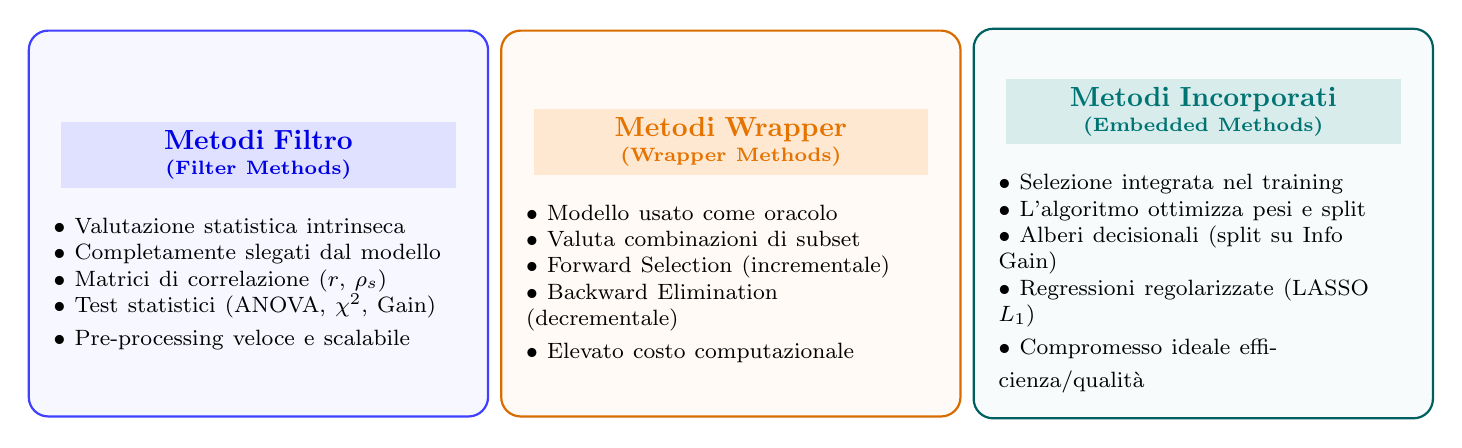
\begin{tikzpicture}[
    card/.style={
        rectangle, rounded corners=7pt, thick,
        inner sep=9pt, text width=5.2cm, minimum height=4.9cm,
        align=left
    },
    filterCard/.style={card, draw=blue!75, fill=blue!3},
    wrapperCard/.style={card, draw=orange!85!black, fill=orange!4},
    embedCard/.style={card, draw=teal!75!black, fill=teal!3}
]
    % --- 1. Filter Methods ---
    \node[filterCard] (filter) at (0, 0) {
        \begin{center}
        \colorbox{blue!12}{\parbox{4.8cm}{\centering\bfseries\color{blue!90!black} Metodi Filtro\\[1pt]\scriptsize (Filter Methods)}}
        \end{center}
        \vspace{2pt}
        \raggedright\footnotesize
        $\bullet$~Valutazione statistica intrinseca\\
        $\bullet$~Completamente slegati dal modello\\
        $\bullet$~Matrici di correlazione ($r$, $\rho_s$)\\
        $\bullet$~Test statistici (ANOVA, $\chi^2$, Gain)\\
        $\bullet$~Pre-processing veloce e scalabile
    };

    % --- 2. Wrapper Methods ---
    \node[wrapperCard] (wrapper) at (6.0, 0) {
        \begin{center}
        \colorbox{orange!18}{\parbox{4.8cm}{\centering\bfseries\color{orange!90!black} Metodi Wrapper\\[1pt]\scriptsize (Wrapper Methods)}}
        \end{center}
        \vspace{2pt}
        \raggedright\footnotesize
        $\bullet$~Modello usato come oracolo\\
        $\bullet$~Valuta combinazioni di subset\\
        $\bullet$~Forward Selection (incrementale)\\
        $\bullet$~Backward Elimination (decrementale)\\
        $\bullet$~Elevato costo computazionale
    };

    % --- 3. Embedded Methods ---
    \node[embedCard] (embed) at (12.0, 0) {
        \begin{center}
        \colorbox{teal!15}{\parbox{4.8cm}{\centering\bfseries\color{teal!90!black} Metodi Incorporati\\[1pt]\scriptsize (Embedded Methods)}}
        \end{center}
        \vspace{2pt}
        \raggedright\footnotesize
        $\bullet$~Selezione integrata nel training\\
        $\bullet$~L'algoritmo ottimizza pesi e split\\
        $\bullet$~Alberi decisionali (split su Info Gain)\\
        $\bullet$~Regressioni regolarizzate (LASSO $L_1$)\\
        $\bullet$~Compromesso ideale efficienza/qualità
    };
\end{tikzpicture}%
}
\caption{Confronto schematico tra le tre famiglie di selezione delle feature: Filter, Wrapper ed Embedded.}
\label{fig:feature-selection-methods}
\end{figure}

\subsection{Strategie Wrapper}
Dato che lo spazio di ricerca esaustivo tra tutti i possibili sottoinsiemi di $p$ feature ha cardinalità $2^p$ (per $p=20$ esistono già oltre 1 milione di combinazioni), i metodi Wrapper adottano euristiche greedy:
\begin{itemize}
    \item \textbf{Forward Selection:} Si parte dall'insieme vuoto $\emptyset$. Ad ogni iterazione si valuta l'aggiunta di ciascuna feature residua e si include quella che apporta il massimo incremento di accuratezza al modello. L'algoritmo si arresta quando l'incremento prestazionale scende sotto una soglia prefissata.
    \item \textbf{Backward Elimination:} Si parte dall'insieme completo di tutte le $p$ feature. Ad ogni iterazione si rimuove la feature la cui esclusione provoca il minor decremento (o addirittura un miglioramento) nelle performance del modello.
\end{itemize}

---

\section{Creazione di Feature (Feature Creation)}

La \textbf{creazione di nuove feature} consiste nella definizione di attributi sintetici capaci di catturare le correlazioni o le proprietà rilevanti del fenomeno in modo molto più efficace ed esplicito rispetto alle feature grezze:

\begin{itemize}
    \item \textbf{Feature Construction guidata dal dominio:} Combinazione algebrica di variabili con significato semantico.
    \begin{example}[Indice di Efficienza del Lavoratore]
    In un'analisi di produttività aziendale, un dipendente è descritto da: compiti completati mensilmente, ore lavorate mensili e tempo standard stimato per completare ciascun compito. Invece di usare i tre valori grezzi separatamente, si introduce l'attributo aggregato:
    \begin{equation}
    \text{Efficienza} = \frac{\text{Ore effettivamente impiegate per completare i task}}{\text{Ore standard mediamente stimate per completare i task}}
    \end{equation}
    \end{example}
    \item \textbf{Feature da Dati Non Strutturati (Computer Vision):} Nelle immagini, i valori grezzi dei singoli pixel contigui non sono adatti direttamente agli algoritmi lineari di classificazione. Si estraggono feature ad alto livello (aree a forte gradiente di contrasto, densità di bordi, istogrammi di colore, mappe di calore di occhi e naso per il riconoscimento facciale).
    \item \textbf{Feature Projection (Proiezione):} Trasformazione matematica globale dallo spazio originale $\mathbb{R}^p$ a un sottospazio $\mathbb{R}^k$ ($k < p$). Tra i metodi lineari principali figurano la \textbf{Principal Component Analysis (PCA)} e la \textbf{Singular Value Decomposition (SVD)}; tra i metodi non lineari e supervisionati rientrano la \textit{Linear Discriminant Analysis} (LDA), la \textit{Non-Negative Matrix Factorization} (NMF) e gli \textit{Autoencoder} neurali.
\end{itemize}

---

\section{Principal Component Analysis (PCA)}

La \textbf{Principal Component Analysis} (PCA) è la tecnica non supervisionata fondamentale per la riduzione lineare della dimensionalità.

\subsection{Intuizione Geometrica e Obiettivi}
Nelle applicazioni reali le feature numeriche sono spesso fortemente correlate tra loro. Si pensi a:
\begin{itemize}
    \item Spese di affitto, stipendio mensile e spese per generi alimentari.
    \item Depositi bancari, stipendio e anzianità lavorativa.
\end{itemize}
La PCA determina un nuovo sistema ortogonale di coordinate ruotato rispetto a quello originario, con le seguenti proprietà:
\begin{enumerate}
    \item La \textbf{prima componente principale (PC1)} si sviluppa lungo la direzione dello spazio che massimizza la varianza (dispersione) dei dati proiettati.
    \item La \textbf{seconda componente principale (PC2)} è rigidamente \textbf{ortogonale} a PC1 e, con tale vincolo geometrico, cattura la massima quota della varianza residua.
    \item Ciascuna componente successiva $\text{PC}_i$ è mutuamente ortogonale a tutte le precedenti e massimizza la dispersione rimanente.
\end{enumerate}

\subsection{Procedura Algoritmica Formale in 5 Passi}
Dato un dataset rappresentato da una matrice $\mathbf{D} \in \mathbb{R}^{m \times n}$ con $m$ osservazioni e $n$ attributi continui:

\begin{algorithm}[H]
\caption{Calcolo delle Componenti Principali (PCA)}
\KwInput{Matrice dei dati originaria $\mathbf{D} \in \mathbb{R}^{m \times n}$, numero di componenti desiderate $k \le n$.}
\KwOutput{Matrice trasformata ridotta $\mathbf{Z} \in \mathbb{R}^{m \times k}$.}
\BlankLine
\tcp{Passo 1: Centratura e Standardizzazione}
Calcola la media campionaria di ciascuna colonna $\bar{x}_j = \frac{1}{m}\sum_{i=1}^m x_{ij}$\;
Sottrai la media per ottenere la matrice centrata $\mathbf{C} \in \mathbb{R}^{m \times n}$: $c_{ij} = x_{ij} - \bar{x}_j$\;
(Opzionale/Raccomandato): Dividi per la deviazione standard $s_j$ se le unità di misura differiscono\;
\BlankLine
\tcp{Passo 2: Calcolo della Matrice di Covarianza}
Calcola la matrice di covarianza campionaria $\mathbf{V} \in \mathbb{R}^{n \times n}$:
\begin{equation}
\mathbf{V} = \frac{1}{m-1}\mathbf{C}^T\mathbf{C}
\end{equation}
La matrice $\mathbf{V}$ è quadrata, simmetrica ($v_{ij} = v_{ji}$) e semidefinita positiva. Gli elementi sulla diagonale principale rappresentano le varianze degli $n$ attributi\;
\BlankLine
\tcp{Passo 3: Risoluzione del Problema agli Autovalori}
Determina gli autovettori ortonormali $\mathbf{e}_j$ e i corrispondenti autovalori $\lambda_j$ risolvendo l'equazione caratteristica:
\begin{equation}
\mathbf{V}\mathbf{e}_j = \lambda_j \mathbf{e}_j \quad \text{con } \|\mathbf{e}_j\|_2 = 1
\end{equation}
\BlankLine
\tcp{Passo 4: Ordinamento e Selezione delle $k$ Componenti Principali}
Ordina gli autovalori in ordine decrescente: $\lambda_1 \ge \lambda_2 \ge \cdots \ge \lambda_n \ge 0$\;
Seleziona i primi $k$ autovettori corrispondenti $\{\mathbf{e}_1, \dots, \mathbf{e}_k\}$ e costruisci la matrice di proiezione $\mathbf{P} \in \mathbb{R}^{n \times k}$ avente come colonne gli autovettori scelti\;
\BlankLine
\tcp{Passo 5: Proiezione dei Dati nel Nuovo Spazio}
Proietta la matrice centrata nello spazio a dimensionalità ridotta:
\begin{equation}
\mathbf{Z} = \mathbf{C}\mathbf{P} \in \mathbb{R}^{m \times k}
\end{equation}
\end{algorithm}

\subsection{Significato della Covarianza e degli Autovalori}
\begin{itemize}
    \item \textbf{Segno della Covarianza:} Il segno di $\text{Cov}(x, y)$ indica la direzione della variazione congiunta:
    \begin{itemize}
        \item $\text{Cov}(x, y) > 0$: $x$ e $y$ tendono ad aumentare o diminuire simultaneamente (ad es. ore di studio e voto conseguito).
        \item $\text{Cov}(x, y) < 0$: all'aumentare di $x$, $y$ tende a diminuire.
        \item $\text{Cov}(x, y) \approx 0$: assenza di relazione lineare tra le due variabili.
    \end{itemize}
    \item \textbf{Autovettori e Autovalori:} Gli autovettori individuano le \textbf{direzioni degli assi di massima varianza} (le Componenti Principali). Ciascun autovalore $\lambda_j$ quantifica la quota assoluta di varianza spiegata dalla rispettiva componente $\text{PC}_j$.
    \item \textbf{Rapporto di Varianza Spiegata:} La percentuale di varianza spiegata dalla componente $j$-esima è pari a:
    \begin{equation}
    \text{Explained Variance Ratio}_j = \frac{\lambda_j}{\sum_{i=1}^n \lambda_i}
    \end{equation}
\end{itemize}

\begin{figure}[H]
\centering

\includegraphics[width=0.78\textwidth]{pca_scree_plot.pdf}
\caption{Scree Plot calcolato sulle 4 feature numeriche del dataset Iris. La prima componente principale (PC1) cattura il 73.0\% della varianza globale, mentre con le prime due componenti (PC1 e PC2) si raggiunge il 95.8\% della varianza complessiva, rendendo sufficiente la rappresentazione bidimensionale.}
\label{fig:pca-scree-plot}
\end{figure}

\begin{figure}[H]
\centering

\includegraphics[width=0.82\textwidth]{pca_2d_projection.pdf}
\caption{Proiezione bidimensionale PCA del dataset Iris lungo le prime due componenti principali (PC1 e PC2). Lo spazio originale quadridimensionale viene sintetizzato senza etichette nel pre-processing, preservando la separazione lineare netta della specie Setosa e la differenziazione morfologica tra Versicolor e Virginica.}
\label{fig:pca-2d-projection}
\end{figure}

\subsection{Laboratorio Python: Principal Component Analysis (PCA) e Scree Plot}
\label{subsec:lab-python-pca}
\begin{noteblock}{Esegui questo blocco nel Notebook Interattivo}
\textbf{Notebook:} \href{http://localhost:8888/lab/tree/notebooks/2_feature_engineering_and_data_representation.ipynb}{\texttt{2\_feature\_engineering\_\dots.ipynb}} \hfill \href{http://localhost:8888/lab/tree/notebooks/2_feature_engineering_and_data_representation.ipynb}{\textbf{[Apri su Jupyter Lab]}} \\
\textit{Server locale:} \url{http://localhost:8888} \quad (comando di avvio: \texttt{docker compose up jupyter})
\end{noteblock}
Nel notebook didattico \texttt{2\_feature\_engineering\_\dots.ipynb}, la riduzione di dimensionalit\`a mediante PCA, il calcolo della varianza spiegata e il tracciamento dello Scree Plot sono realizzati con Scikit-learn come illustrato nel Listing~\ref{lst:python-pca}:

\begin{lstlisting}[language=Python, style=code, caption={Esecuzione di PCA, analisi degli autovalori e Scree Plot con Scikit-learn.}, label={lst:python-pca}]
import pandas as pd
import numpy as np
import matplotlib.pyplot as plt
from sklearn.decomposition import PCA

df = pd.read_csv('./data_notebook/data/correct_tips.csv', index_col=0)
numeric_cols = ['total_bill', 'tip', 'size', 'age']
X = df[numeric_cols]

# 1. Istanziazione ed esecuzione della PCA completa
pca = PCA()
X_pca = pca.fit_transform(X)

# 2. Autovalori (varianza spiegata) e percentuale di varianza per componente
eigenvalues = pca.explained_variance_
var_ratio = pca.explained_variance_ratio_
cum_var = np.cumsum(var_ratio)

for i, (eig, ratio, c) in enumerate(zip(eigenvalues, var_ratio, cum_var), 1):
    print(f"PC{i}: Autovalore={eig:.3f} | Varianza={ratio*100:.1f}% | Cumulata={c*100:.1f}%")

# 3. Scree Plot degli autovalori
plt.figure(figsize=(7, 4))
plt.plot(range(1, len(eigenvalues) + 1), eigenvalues, marker='o', linestyle='--', color='b')
plt.title("Scree Plot: Autovalori delle Componenti Principali")
plt.xlabel("Componente Principale")
plt.ylabel("Autovalore (Varianza spiegata)")
plt.grid(True)
plt.show()
\end{lstlisting}

\section{Gestione dei Valori Mancanti e Anomali (Cleaning)}

\subsection{Tipologie e Cause di Valori Anomali}
I dati grezzi contengono frequentemente imperfezioni dovute a malfunzionamento di sensori, rifiuti di risposta in indagini campionarie, errori di digitazione o modifiche strutturali nelle procedure di raccolta:
\begin{itemize}
    \item \textbf{Valori Mancanti (\textit{Missing}):} Campi non pervenuti, omessi o codificati esplicitamente come \texttt{NULL} o \texttt{NaN}.
    \item \textbf{Valori Sconosciuti (\textit{Unknown}):} Campi valorizzati formalmente ma privi di reale significato semantico nel dominio di riferimento.
    \item \textbf{Valori Non Validi (\textit{Invalid}):} Dati che violano i vincoli di integrità del dominio (ad esempio un'età negativa, un punteggio esame superiore al massimo ammissibile o codici fiscali malformati).
\end{itemize}

\subsection{Strategie Metodologiche di Trattamento dei Dati Mancanti}
Nelle applicazioni pratiche di Data Mining, la gestione dei missing value si articola in tre macro-approcci complementari:

\begin{enumerate}
    \item \textbf{Eliminazione (\textit{Data / Attribute Removal}):}
    \begin{itemize}
        \item \textit{Eliminazione delle Istanze (Listwise / Case Deletion):} Rimozione dell'intero record che presenta uno o più attributi nulli. È lecita soltanto se la proporzione di missing è ridottissima ($< 3\div 5\%$) e i valori sono assenti completamente a caso (\textit{Missing Completely at Random} - MCAR). Se l'assenza dipende da altri fattori (es. clienti ad alto reddito che omettono lo stipendio), l'eliminazione introduce una grave distorsione di selezione (\textit{selection bias}).
        \item \textit{Eliminazione dell'Attributo (Feature Deletion):} Rimozione dell'intera colonna. È raccomandata quando l'attributo presenta percentuali di assenza eccessive (superiori al $50\div 60\%$) e non possiede una rilevanza predittiva insostituibile per il task.
        \item \textit{Eliminazione a Coppie (Pairwise Deletion):} Utilizzata nel calcolo di statistiche bivariati (come la covarianza o la matrice di correlazione), escludendo dal calcolo solo le singole coppie che contengono un valore nullo, massimizzando l'impiego dei dati disponibili.
    \end{itemize}

    \item \textbf{Stima e Imputazione dei Valori (\textit{Value Imputation}):}
    \begin{itemize}
        \item \textbf{Sostituzione con Stimatori Globali (Media, Mediana, Moda):}
        La media aritmetica si impiega per variabili numeriche simmetriche; la mediana è lo stimatore raccomandato per distribuzioni asimmetriche con code pesanti e presenza di outlier; la moda si applica alle feature categoriche nominali od ordinali. \textit{Criticità:} riduce artificialmente la varianza della feature e attenua le covarianze tra variabili distinte.
        \item \textbf{Campionamento dalla Distribuzione Empirica:}
        Il valore mancante viene rimpiazzato estraendo casualmente un'osservazione secondo la distribuzione di probabilità empirica dei valori validi osservati nel dataset. \textit{Vantaggio:} preserva intatta la dispersione originale, la varianza e l'istogramma empirico della feature.
        \item \textbf{Imputazione Stratificata per Segmento o Cluster:}
        I dati vengono partizionati in gruppi omogenei (ad esempio per classe target, professione o tramite un algoritmo di clustering come k-means); il missing viene quindi rimpiazzato dalla mediana o media calcolata esclusivamente all'interno dello strato o cluster di appartenenza (es. stimare lo stipendio mancante usando la mediana della sola qualifica professionale del soggetto).
        \item \textbf{Modello Predittivo Supervisionato:}
        L'attributo affetto da valori mancanti viene trattato come variabile target $Y$. Si addestra un modello predittivo (albero di decisione, regressione o $k$-NN) impiegando gli attributi completi come predittori per stimare il valore incognito con la massima accuratezza contestuale.
    \end{itemize}

    \item \textbf{Tolleranza e Gestione Algoritmica Diretta (\textit{Ignore Missing Values}):}
    Molti algoritmi avanzati gestiscono direttamente i missing durante la fase di apprendimento, senza richiedere una manipolazione preventiva dei dati:
    \begin{itemize}
        \item \textit{Alberi di Decisione (es. C4.5):} Nelle valutazioni dei nodi, l'algoritmo distribuisce le istanze con valore mancante proporzionalmente su tutti i rami figli in base alle frequenze relative osservate, oppure crea un ramo dedicato (\textit{missing branch}).
        \item \textit{Regole Associative:} Nelle matrici transazionali binarie, un valore non presente corrisponde intrinsecamente all'assenza dell'item ($0$), rendendo l'omissione parte naturale della semantica del modello.
    \end{itemize}
\end{enumerate}

\begin{figure}[H]
\centering
\resizebox{0.98\linewidth}{!}{%
\begin{tikzpicture}[
    header/.style={rectangle, draw=blue!60, fill=blue!12, minimum width=0.95cm, minimum height=0.50cm, font=\scriptsize\bfseries, text=blue!90!black, align=center},
    cell/.style={rectangle, draw=gray!40, fill=white, minimum width=0.95cm, minimum height=0.46cm, font=\scriptsize, align=center},
    nanCell/.style={rectangle, draw=red!70, fill=red!18, minimum width=0.95cm, minimum height=0.46cm, font=\scriptsize\bfseries, text=red!80!black, align=center},
    impCell/.style={rectangle, draw=teal!70, fill=teal!18, minimum width=0.95cm, minimum height=0.46cm, font=\scriptsize\bfseries, text=teal!90!black, align=center},
    boxTitle/.style={font=\small\bfseries, text=gray!90!black, align=center},
    arrowLbl/.style={font=\scriptsize\bfseries, fill=white, inner sep=2.5pt, rounded corners=3pt}
]
    % --- Matrice Originale ---
    \node[boxTitle] (t0) at (0, 2.2) {Dataset con Dati Mancanti};
    \node[header] (h1) at (-0.95, 1.5) {$A_1$};
    \node[header] (h2) at (0, 1.5) {$A_2$};
    \node[header] (h3) at (0.95, 1.5) {$A_3$};

    \node[cell] at (-0.95, 0.95) {24}; \node[cell] at (0, 0.95) {1.8}; \node[cell] at (0.95, 0.95) {50};
    \node[cell] at (-0.95, 0.45) {31}; \node[nanCell] at (0, 0.45) {NaN}; \node[cell] at (0.95, 0.45) {65};
    \node[cell] at (-0.95, -0.05) {45}; \node[cell] at (0, -0.05) {2.3}; \node[cell] at (0.95, -0.05) {80};
    \node[cell] at (-0.95, -0.55) {19}; \node[nanCell] at (0, -0.55) {NaN}; \node[nanCell] at (0.95, -0.55) {NaN};
    \node[cell] at (-0.95, -1.05) {29}; \node[cell] at (0, -1.05) {1.5}; \node[cell] at (0.95, -1.05) {55};

    \draw[rounded corners=6pt, draw=blue!40, thick, fill=blue!1, fill opacity=0.3] (-1.65, -1.40) rectangle (1.65, 1.85);

    % --- Frecce alle 3 Strategie ---
    \draw[-Stealth, line width=1.3pt, color=orange!85!black] (1.75, 0.95) -- (4.4, 2.85) 
        node[midway, above=2pt, sloped, arrowLbl, draw=orange!40, text=orange!90!black] {Listwise Deletion};
        
    \draw[-Stealth, line width=1.3pt, color=red!80!black] (1.75, 0.0) -- (4.4, 0.0) 
        node[midway, above=2pt, arrowLbl, draw=red!40, text=red!85!black] {Feature Deletion};
        
    \draw[-Stealth, line width=1.3pt, color=teal!85!black] (1.75, -0.95) -- (4.4, -2.85) 
        node[midway, below=2pt, sloped, arrowLbl, draw=teal!40, text=teal!90!black] {Value Imputation};

    % --- Strategia 1: Listwise Deletion ---
    \begin{scope}[shift={(6.7, 2.95)}]
        \draw[rounded corners=7pt, draw=orange!55, fill=orange!3, thick] (-2.1, -1.35) rectangle (10.6, 1.35);
        \node[font=\footnotesize\bfseries, text=orange!95!black, anchor=west] at (-1.9, 0.98) {1. Eliminazione Record (\textit{Listwise Deletion})};
        
        \node[header] at (-1.1, 0.30) {$A_1$}; \node[header] at (-0.15, 0.30) {$A_2$}; \node[header] at (0.8, 0.30) {$A_3$};
        \node[cell] at (-1.1, -0.20) {24}; \node[cell] at (-0.15, -0.20) {1.8}; \node[cell] at (0.8, -0.20) {50};
        \node[cell] at (-1.1, -0.70) {45}; \node[cell] at (-0.15, -0.70) {2.3}; \node[cell] at (0.8, -0.70) {80};
        
        \draw[gray!30, line width=0.7pt] (1.45, -1.05) -- (1.45, 0.75);

        \node[font=\scriptsize, text=gray!85!black, anchor=west, align=left, text width=8.6cm] at (1.65, -0.20) {
            $\bullet$ Scarta ogni riga contenente almeno un missing (valore NaN)\\[5pt]
            $\bullet$ Ammissibile solo se i missing sono trascurabili ($< 3\div 5\%$)\\[5pt]
            $\bullet$ Rischio elevato di \textbf{selection bias} se i dati non sono MCAR
        };
    \end{scope}

    % --- Strategia 2: Feature Deletion ---
    \begin{scope}[shift={(6.7, 0.0)}]
        \draw[rounded corners=7pt, draw=red!55, fill=red!3, thick] (-2.1, -1.35) rectangle (10.6, 1.35);
        \node[font=\footnotesize\bfseries, text=red!90!black, anchor=west] at (-1.9, 0.98) {2. Eliminazione Attributo (\textit{Feature Deletion})};
        
        \node[header] at (-0.65, 0.30) {$A_1$}; \node[header] at (0.35, 0.30) {$A_3$};
        \node[cell] at (-0.65, -0.20) {24}; \node[cell] at (0.35, -0.20) {50};
        \node[cell] at (-0.65, -0.70) {31}; \node[cell] at (0.35, -0.70) {65};
        
        \draw[gray!30, line width=0.7pt] (1.45, -1.05) -- (1.45, 0.75);

        \node[font=\scriptsize, text=gray!85!black, anchor=west, align=left, text width=8.6cm] at (1.65, -0.20) {
            $\bullet$ Rimuove l'intera colonna incompleta ($A_2$) dalle feature\\[5pt]
            $\bullet$ Consigliata se il tasso di missing è critico ($> 50\div 60\%$)\\[5pt]
            $\bullet$ Preserva integralmente tutte le altre osservazioni del dataset
        };
    \end{scope}

    % --- Strategia 3: Value Imputation ---
    \begin{scope}[shift={(6.7, -2.95)}]
        \draw[rounded corners=7pt, draw=teal!55, fill=teal!3, thick] (-2.1, -1.35) rectangle (10.6, 1.35);
        \node[font=\footnotesize\bfseries, text=teal!90!black, anchor=west] at (-1.9, 0.98) {3. Imputazione dei Valori (\textit{Value Imputation})};
        
        \node[header] at (-1.1, 0.30) {$A_1$}; \node[header] at (-0.15, 0.30) {$A_2$}; \node[header] at (0.8, 0.30) {$A_3$};
        \node[cell] at (-1.1, -0.20) {31}; \node[impCell] at (-0.15, -0.20) {1.9}; \node[cell] at (0.8, -0.20) {65};
        \node[cell] at (-1.1, -0.70) {19}; \node[impCell] at (-0.15, -0.70) {1.9}; \node[impCell] at (0.8, -0.70) {58};
        
        \draw[gray!30, line width=0.7pt] (1.45, -1.05) -- (1.45, 0.75);

        \node[font=\scriptsize, text=gray!85!black, anchor=west, align=left, text width=8.6cm] at (1.65, -0.20) {
            $\bullet$ Sostituzione con media, mediana o modello predittivo\\[5pt]
            $\bullet$ \textbf{Campionamento empirico}: preserva la varianza originaria\\[5pt]
            $\bullet$ \textbf{Imputazione stratificata}: preserva le differenze tra cluster
        };
    \end{scope}
\end{tikzpicture}%
}
\caption{Panoramica schematica delle strategie di gestione dei missing value: eliminazione di record o attributi versus imputazione.}
\label{fig:missing-values-strategies}
\end{figure}

\subsection{Rilevamento e Trattamento di Outlier Univariati}
Nel pre-processing si utilizzano due regole formali (Figura~\ref{fig:outlier-detection-methods}):
\begin{enumerate}
    \item \textbf{Regola del Range Interquartile (Tukey IQR Fences):}
    \begin{equation}
    \text{IQR} = Q_3 - Q_1, \quad L = Q_1 - 1.5 \times \text{IQR}, \quad U = Q_3 + 1.5 \times \text{IQR}
    \end{equation}
    Un'osservazione $x$ è classificata come outlier se $x < L$ oppure $x > U$.
    \begin{itemize}
        \item \textit{Sostituzione (Winsorizing):} I valori inferiori a $L$ vengono sostituiti con $L$, quelli superiori a $U$ vengono sostituiti con $U$.
        \item \textit{Sostituzione con la mediana:} Il valore anomalo viene rimpiazzato direttamente con $Q_2$.
    \end{itemize}
    \item \textbf{Approccio Parametrico basato su Z-Score:}
    Per dati distribuiti approssimativamente secondo una normale:
    \begin{itemize}
        \item Il 95\% delle osservazioni ricade in $[ -1.96, +1.96 ]$.
        \item Il 99\% delle osservazioni ricade in $[ -2.58, +2.58 ]$.
        \item La soglia canonica per identificare valori anomali estremi è posta a $|z| > 3.29$ (probabilità $< 0.1\%$).
        \item \textit{Sostituzione del valore anomalo:} Si tronca il valore $x$ al punteggio corrispondente a $z = \pm 3.0$ (estremità della campana gaussiana), oppure si sostituisce con il valore medio ($z = 0$).
    \end{itemize}
\end{enumerate}

\begin{figure}[H]
\centering
\resizebox{0.96\linewidth}{!}{%
\begin{tikzpicture}[
    outlierPt/.style={circle, draw=red!80!black, fill=red!45, inner sep=2.2pt, thick},
    whisker/.style={line width=1.1pt, draw=blue!85!black},
    boxStyle/.style={rectangle, draw=blue!85!black, line width=1.2pt, fill=blue!10}
]
    % --- SEZIONE A: BOXPLOT TUKEY ---
    \node[anchor=west, font=\small\bfseries, text=blue!90!black] at (-6.8, 4.4) {A) Regola Non Parametrica del Range Interquartile (Tukey IQR Fences)};

    % Asse orizzontale
    \draw[-Stealth, line width=0.8pt, color=gray!70] (-6.8, 1.8) -- (6.8, 1.8) node[right, font=\scriptsize] {$x$};
    \foreach \x in {-5.5, -3.5, -1.0, 0.5, 2.0, 4.5, 5.5} {
        \draw[gray!60] (\x, 1.7) -- (\x, 1.9);
    }
    
    % Etichette sotto l'asse alternate per leggibilità
    \node[below=3pt, font=\scriptsize\bfseries, text=red!80!black] at (-3.5, 1.7) {$L = Q_1 - 1.5\,\text{IQR}$};
    \node[below=3pt, font=\scriptsize\bfseries, text=red!80!black] at (4.5, 1.7) {$U = Q_3 + 1.5\,\text{IQR}$};
    \node[below=3pt, font=\scriptsize] at (-1.0, 1.7) {$Q_1$};
    \node[below=3pt, font=\scriptsize\bfseries, text=blue!90!black] at (0.5, 1.7) {Mediana ($Q_2$)};
    \node[below=3pt, font=\scriptsize] at (2.0, 1.7) {$Q_3$};

    % Box
    \draw[boxStyle] (-1.0, 2.3) rectangle (2.0, 3.3);
    \draw[line width=1.6pt, draw=blue!95!black] (0.5, 2.3) -- (0.5, 3.3);

    % Staffa IQR SOPRA il box
    \draw[decorate, decoration={brace, amplitude=4pt}, line width=0.8pt, draw=blue!80!black] (-1.0, 3.4) -- (2.0, 3.4) 
        node[midway, above=4pt, font=\scriptsize\bfseries, text=blue!85!black] {$\text{IQR} = Q_3 - Q_1$};

    % Baffi (Whiskers)
    \draw[whisker] (-1.0, 2.8) -- (-3.5, 2.8);
    \draw[whisker] (-3.5, 2.5) -- (-3.5, 3.1);
    \draw[whisker] (2.0, 2.8) -- (4.5, 2.8);
    \draw[whisker] (4.5, 2.5) -- (4.5, 3.1);

    % Punti Outlier
    \node[outlierPt] at (-4.8, 2.8) {};
    \node[outlierPt] at (-5.6, 2.8) {};
    \node[outlierPt] at (5.2, 2.8) {};
    \node[outlierPt] at (6.0, 2.8) {};

    \node[font=\scriptsize\bfseries, text=red!80!black] at (-5.2, 3.5) {Outlier ($x < L$)};
    \node[font=\scriptsize\bfseries, text=red!80!black] at (5.6, 3.5) {Outlier ($x > U$)};

    % Frecce Winsorizing
    \draw[-Stealth, line width=1pt, draw=teal!80!black, dashed] (-5.2, 2.4) to[bend left=18] 
        node[midway, below=1pt, font=\tiny\bfseries, text=teal!90!black] {Winsorizing $\to L$} (-3.55, 2.4);
    \draw[-Stealth, line width=1pt, draw=teal!80!black, dashed] (5.6, 2.4) to[bend right=18] 
        node[midway, below=1pt, font=\tiny\bfseries, text=teal!90!black] {Winsorizing $\to U$} (4.55, 2.4);

    % --- SEPARATORE ---
    \draw[dashed, color=gray!30] (-6.8, 0.8) -- (6.8, 0.8);

    % --- SEZIONE B: CURVA NORMALE Z-SCORE ---
    \node[anchor=west, font=\small\bfseries, text=purple!85!black] at (-6.8, 0.4) {B) Regola Parametrica Z-Score (Distribuzione Gaussiana $\mathcal{N}(\mu, \sigma^2)$)};

    % Asse orizzontale z-score (a y = -3.0)
    \draw[-Stealth, line width=0.8pt, color=gray!70] (-6.8, -3.0) -- (6.8, -3.0) node[right, font=\scriptsize] {$z$};

    % Area 95% (da -1.96 a +1.96)
    \fill[teal!15] (-2.0, -3.0) .. controls (-1.0, -2.9) and (-0.8, -1.0) .. (0, -0.6)
                                .. controls (0.8, -1.0) and (1.0, -2.9) .. (2.0, -3.0) -- cycle;

    % Area Outlier Sinistra (z < -3.29)
    \fill[red!30] (-6.2, -3.0) -- (-3.3, -3.0) .. controls (-3.8, -2.94) and (-4.8, -2.98) .. (-6.2, -3.0) -- cycle;
    % Area Outlier Destra (z > 3.29)
    \fill[red!30] (3.3, -3.0) .. controls (4.8, -2.98) and (3.8, -2.94) .. (6.2, -3.0) -- (3.3, -3.0) -- cycle;

    % Curva Gaussiana completa disegnata con Bézier smooth
    \draw[line width=1.4pt, color=purple!85!black] 
        (-6.2, -3.0) .. controls (-4.5, -2.98) and (-3.0, -2.8) .. (-2.0, -2.2)
                     .. controls (-1.2, -1.6) and (-0.6, -0.7) .. (0, -0.6)
                     .. controls (0.6, -0.7) and (1.2, -1.6) .. (2.0, -2.2)
                     .. controls (3.0, -2.8) and (4.5, -2.98) .. (6.2, -3.0);

    % Linee verticali
    \draw[line width=0.9pt, color=purple!80!black, dashed] (0, -3.0) -- (0, -0.6) 
        node[above=2pt, font=\scriptsize\bfseries] {$\mu$ ($z=0$)};
    \draw[line width=0.8pt, color=teal!70!black, dotted] (-2.0, -3.0) -- (-2.0, -2.2);
    \draw[line width=0.8pt, color=teal!70!black, dotted] (2.0, -3.0) -- (2.0, -2.2);
    \draw[line width=1pt, color=red!70!black, dashed] (-3.3, -3.0) -- (-3.3, -2.85);
    \draw[line width=1pt, color=red!70!black, dashed] (3.3, -3.0) -- (3.3, -2.85);

    % Etichette
    \node[font=\scriptsize\bfseries, text=teal!90!black] at (0, -1.6) {95\% della popolazione};
    \node[font=\tiny, text=gray!80!black] at (0, -2.0) {($-1.96 \le z \le +1.96$)};

    \node[below=2pt, font=\scriptsize\bfseries, text=red!80!black] at (-3.3, -3.0) {$-3.29$};
    \node[below=2pt, font=\scriptsize\bfseries, text=red!80!black] at (3.3, -3.0) {$+3.29$};
    \node[below=2pt, font=\scriptsize, text=teal!80!black] at (-2.0, -3.0) {$-1.96$};
    \node[below=2pt, font=\scriptsize, text=teal!80!black] at (2.0, -3.0) {$+1.96$};
    \node[below=2pt, font=\scriptsize\bfseries] at (0, -3.0) {$0$};

    \node[font=\scriptsize\bfseries, text=red!85!black, align=center] at (-4.7, -1.8) {Outlier Estremi\\$|z| > 3.29$\\($p < 0.1\%$)};
    \node[font=\scriptsize\bfseries, text=red!85!black, align=center] at (4.7, -1.8) {Outlier Estremi\\$|z| > 3.29$\\($p < 0.1\%$)};
\end{tikzpicture}%
}
\caption{Confronto tra i metodi di rilevamento degli outlier univariati: Regola di Tukey basata su IQR e approccio parametrico basato su Z-Score.}
\label{fig:outlier-detection-methods}
\end{figure}

\FloatBarrier

---

\section{Discretizzazione e Binarizzazione}

\subsection{Definizione e Vantaggi della Discretizzazione}
La \textbf{discretizzazione} è il processo di trasformazione di un attributo continuo in un attributo ordinale discreto, mappando un insieme infinito di valori reali in un numero finito $k$ di categorie o intervalli (\textit{bins}).

\begin{itemize}
    \item \textbf{Semplicità interpretativa:} Trasforma serie numeriche sparse in classi leggibili (es. $\{ \text{Giovane}, \text{Adulto}, \text{Anziano} \}$).
    \item \textbf{Robustezza e stabilità:} Attenua l'influenza di piccoli errori di misurazione e di singoli outlier.
    \item \textbf{Requisito algoritmico:} Alcuni algoritmi (come le regole associative e determinati modelli bayesiani o ad albero) richiedono esplicitamente variabili categoriali discrete.
\end{itemize}

\subsection{Discretizzazione Non Supervisionata (Unsupervised Binning)}
Si applica quando non si dispone di un'etichetta target di classe per guidare la scelta dei confini:

\begin{enumerate}
    \item \textbf{Natural Binning (Equal-Width Binning):}
    Divide l'escursione totale dei dati in $k$ intervalli di ampiezza costante $\delta$:
    \begin{equation}
    \delta = \frac{x_{\max} - x_{\min}}{k}
    \end{equation}
    Un elemento $x_j$ appartiene alla classe $i$ ($i \in \{0, \dots, k-1\}$) se:
    \begin{equation}
    x_j \in [x_{\min} + i\delta, \; x_{\min} + (i+1)\delta)
    \end{equation}
    \textit{Criticità:} Se la distribuzione presenta asimmetria o outlier estremi, la maggior parte dei campioni si concentra in pochissimi intervalli, lasciando i restanti bin vuoti o quasi disabitati.
    
    \item \textbf{Equal-Frequency (Quantile) Binning:}
    Ordina gli elementi e definisce $k$ intervalli tali che ciascuno contenga all'incirca lo stesso numero di osservazioni $f = \frac{N}{k}$:
    Un elemento $x_i$ (nell'ordinamento crescente con indice $i \in \{0, \dots, N-1\}$) appartiene alla classe $j$ se:
    \begin{equation}
    j \times f \le i < (j+1) \times f
    \end{equation}
    \textit{Vantaggio:} Massimizza l'entropia della partizione ed evita bin vuoti.
\end{enumerate}

\subsection{Criteri per la Scelta del Numero Ottimale di Classi}
La scelta del parametro $k$ determina il compromesso tra fedeltà distributiva e leggibilità:
\begin{itemize}
    \item Se $k$ è troppo piccolo: perdita marcata di informazione sulla reale forma distributiva.
    \item Se $k$ è troppo grande: eccessiva frammentazione con forte rumore campionario.
\end{itemize}
I criteri analitici raccomandati in letteratura statistica sono:
\begin{itemize}
    \item \textbf{Regola di Sturges (1929):} Adatta per distribuzioni simmetriche unimodali:
    \begin{equation}
    k = 1 + \frac{10}{3} \log_{10}(N) \approx 1 + 3.322 \log_{10}(N) = 1 + \log_2(N)
    \end{equation}
    \item \textbf{Regola di Scott (1979):} Calcola direttamente l'ampiezza ottimale dei bin $h$ in funzione della deviazione standard $s$:
    \begin{equation}
    h = \frac{3.5 \times s}{\sqrt[3]{N}}
    \end{equation}
\end{itemize}

\subsection{Discretizzazione Supervisionata: Metodo Basato sull'Entropia}
Nel contesto della classificazione supervisionata, la discretizzazione di una feature continua $X$ ha come obiettivo esplicito la \textbf{massimizzazione della purezza delle classi} all'interno di ciascun intervallo, minimizzando l'entropia condizionata rispetto all'etichetta $Y$.
L'algoritmo procede solitamente con un approccio greedy bipartizionale:
\begin{enumerate}
    \item Si valuta ogni possibile valore di soglia $T$ lungo il dominio ordinato di $X$.
    \item Per ogni split nei due sotto-intervalli $S_1 = \{x \le T\}$ e $S_2 = \{x > T\}$, si calcola l'entropia pesata:
    \begin{equation}
    E(X, T) = \frac{|S_1|}{|S|} \text{Entropy}(S_1) + \frac{|S_2|}{|S|} \text{Entropy}(S_2)
    \end{equation}
    dove l'entropia di un sottoinsieme $S$ rispetto alle $C$ classi è $\text{Entropy}(S) = -\sum_{c=1}^C p_c \log_2(p_c)$.
    \item Si seleziona la soglia $T^*$ che minimizza $E(X, T)$ (massimizzando il Guadagno Informativo o \textit{Information Gain}).
    \item Il procedimento viene iterato ricorsivamente sull'intervallo con entropia peggiore (più impuro) finché non si raggiunge il numero prefissato di classi o un criterio di stop basato sul principio del Minimum Description Length (MDL).
\end{enumerate}

\subsection{Binarizzazione}
La \textbf{binarizzazione} mappa un attributo continuo (previa discretizzazione) o categorico in una o più variabili binarie ($0$ o $1$). In letteratura e nei sistemi di Data Mining si distinguono due paradigmi principali:

\begin{enumerate}
    \item \textbf{Codifica Binaria Compatta Posizionale (\textit{Integer-to-Binary}):}
    Un attributo categorico con $m$ modalità distinte viene mappato su interi $\{0, 1, \dots, m-1\}$ e convertito nella relativa rappresentazione binaria posizionale impiegando $k = \lceil \log_2(m) \rceil$ bit.
    \begin{itemize}
        \item \textit{Esempio:} Per un attributo con $m=4$ stati (es.~Rosso, Blu, Verde, Giallo), sono necessari $\lceil \log_2(4) \rceil = 2$ bit:
        \begin{equation}
        \text{Rosso} \to 00_2, \quad \text{Blu} \to 01_2, \quad \text{Verde} \to 10_2, \quad \text{Giallo} \to 11_2
        \end{equation}
        \item \textit{Criticità ed Effetti Collaterali:} Sebbene riduca al minimo il numero di colonne, questa codifica introduce \textbf{relazioni metriche e correlazioni spurie}:
        \begin{itemize}
            \item \textit{Distanza distorta:} La distanza di Hamming tra Rosso ($00$) e Blu ($01$) è pari a $1$, mentre tra Rosso ($00$) e Giallo ($11$) è pari a $2$. Il modello apprende erroneamente che Giallo è ``più lontano'' da Rosso rispetto a Blu, falsando il significato originario di una variabile nominale priva di ordinamento.
            \item \textit{Falsi pattern di correlazione:} La condivisione accidentale di singoli bit (es. il primo bit uguale a $1$ per Verde e Giallo) induce correlazioni numeriche artificiali che ingannano gli stimatori di machine learning.
        \end{itemize}
    \end{itemize}

    \item \textbf{Binarizzazione Asimmetrica / One-Hot Encoding:}
    Per un attributo a $m$ modalità distinte, si introducono $m$ distinte variabili indicatrici binarie $x_1, \dots, x_m$, dove $x_j = 1$ se l'osservazione possiede la modalità $j$, e $x_j = 0$ altrimenti (Tabella~\ref{tab:binarization-example}).
    \begin{itemize}
        \item \textit{Proprietà Geometriche:} Tutte le modalità risultano ortogonali nello spazio euclideo $\mathbb{R}^m$ e reciprocamente equidistanti ($\|\mathbf{x}_i - \mathbf{x}_j\|_2 = \sqrt{2}$ per $i \ne j$), preservando fedelmente l'assoluta assenza di gerarchia della variabile nominale.
        \item \textit{Requisito Fondamentale per l'Association Analysis (Regole Associative):}
        Negli algoritmi per pattern frequenti (come Apriori o FP-Growth), i record sono modellati come insiemi di item binari asimmetrici:
        \begin{itemize}
            \item La presenza dell'item ($1$, ad esempio l'acquisto di un determinato prodotto) possiede valore semantico discriminante e contribuisce al calcolo di supporto e confidenza.
            \item L'assenza dell'item ($0$) costituisce lo stato naturale di sfondo non informativo (in un catalogo di $50\,000$ articoli, ogni transazione contiene pochissimi oggetti).
            \item Con variabili binarie simmetriche o codifiche compatte posizionali, gli algoritmi estrarrebbero un numero sterminato di associazioni prive di valore pratico basate sulla non-compresenza simultanea (es. ``chi non compra caviale non compra elicotteri''). La One-Hot encoding garantisce che ciascun valore sia trattato come un item asimmetrico indipendente.
        \end{itemize}
    \end{itemize}
\end{enumerate}

\begin{table}[H]
\centering
\small
\begin{tabular}{lcccccc}
\toprule
\textbf{Valore Categorico} & \textbf{Indice} & $x_1$ & $x_2$ & $x_3$ & $x_4$ & $x_5$ \\
\midrule
awful  & 0 & 1 & 0 & 0 & 0 & 0 \\
poor   & 1 & 0 & 1 & 0 & 0 & 0 \\
OK     & 2 & 0 & 0 & 1 & 0 & 0 \\
good   & 3 & 0 & 0 & 0 & 1 & 0 \\
great  & 4 & 0 & 0 & 0 & 0 & 1 \\
\bottomrule
\end{tabular}
\caption{Conversione di un attributo qualitativo con $m=5$ modalità in $5$ attributi binari asimmetrici (One-Hot Encoding).}
\label{tab:binarization-example}
\end{table}

\subsection{Laboratorio Python: Discretizzazione ed Encoding Categorico}
\label{subsec:lab-python-encoding}
\begin{noteblock}{Esegui questo blocco nel Notebook Interattivo}
\textbf{Notebook:} \href{http://localhost:8888/lab/tree/notebooks/2_feature_engineering_and_data_representation.ipynb}{\texttt{2\_feature\_engineering\_\dots.ipynb}} \hfill \href{http://localhost:8888/lab/tree/notebooks/2_feature_engineering_and_data_representation.ipynb}{\textbf{[Apri su Jupyter Lab]}} \\
\textit{Server locale:} \url{http://localhost:8888} \quad (comando di avvio: \texttt{docker compose up jupyter})
\end{noteblock}
Nel notebook didattico \texttt{2\_feature\_engineering\_\dots.ipynb}, la discretizzazione numerica e le strategie di codifica categorica (One-Hot Encoding e Target Encoding) sono implementate con Scikit-learn come mostrato nel Listing~\ref{lst:python-encoding}:

\begin{lstlisting}[language=Python, style=code, caption={Discretizzazione con KBinsDiscretizer ed Encoding (One-Hot e Target Encoding) con Scikit-learn.}, label={lst:python-encoding}]
import pandas as pd
from sklearn.preprocessing import KBinsDiscretizer, OneHotEncoder, TargetEncoder

df = pd.read_csv('./data_notebook/data/correct_tips.csv', index_col=0)

# 1. Discretizzazione continua -> ordinale (Equal-Width vs Equal-Frequency)
kbins_uniform = KBinsDiscretizer(n_bins=4, encode='ordinal', strategy='uniform')
df['bill_uniform'] = kbins_uniform.fit_transform(df[['total_bill']])

kbins_quantile = KBinsDiscretizer(n_bins=4, encode='ordinal', strategy='quantile')
df['bill_quantile'] = kbins_quantile.fit_transform(df[['total_bill']])
print("Conteggi bin uniformi:\n", df['bill_uniform'].value_counts())

# 2. One-Hot Encoding per variabili categoriche nominali
ohe = OneHotEncoder(handle_unknown='ignore', sparse_output=False)
ohe_day = ohe.fit_transform(df[['day']])
df_ohe = pd.DataFrame(ohe_day, columns=ohe.get_feature_names_out(['day']))
print("Feature One-Hot generate:\n", df_ohe.head(3))

# 3. Target Encoding supervisionato
target_encoder = TargetEncoder(smooth="auto")
# Calcola la stima condizionata lisciata della variabile target numerica ('tip')
df['day_target_encoded'] = target_encoder.fit_transform(df[['day']], df['tip'])
print(df[['day', 'day_target_encoded']].drop_duplicates())
\end{lstlisting}

\FloatBarrier

---

\section{Trasformazione degli Attributi e Stabilizzazione della Varianza}

\subsection{Motivazioni e Proprietà Formali}
Una trasformazione di attributo è una funzione $T: \mathcal{X} \to \mathcal{Y}$ che associa a ciascun valore originario $x$ un nuovo valore sostitutivo $y = T(x)$.
Le proprietà desiderabili di una buona trasformazione $T$ sono:
\begin{enumerate}
    \item \textbf{Conservazione dell'informazione essenziale:} Preservare l'ordinamento naturale degli oggetti ($x_a < x_b \implies T(x_a) < T(x_b)$ per trasformazioni strettamente monotone).
    \item \textbf{Risoluzione di criticità distributive:} Rendere le distribuzioni unimodali e simmetriche, eliminare code pesanti ed eliminare la dispersione non omogenea.
    \item \textbf{Linearizzazione delle relazioni:} Rendere approssimativamente lineari relazioni bivariati originariamente esponenziali o quadratiche.
    \item \textbf{Regolarità analitica:} Funzioni continue, differenziabili e invertibili su tutto il dominio applicativo.
\end{enumerate}

\subsection{Famiglia delle Trasformazioni Esponenziali e Logaritmiche}
La forma generale parametrica di trasformazione per $x > 0$ è definita da:
\begin{equation}
T_p(x) = \begin{cases}
a x^p + b & \text{se } p \ne 0 \\
c \log(x) + d & \text{se } p = 0
\end{cases}
\end{equation}
In base al parametro reale $p$:
\begin{itemize}
    \item \textbf{Trasformazione Lineare ($p=1$):} Preserva integralmente forma, skewness e correlazioni; consente il cambio di scala o di unità di misura:
    \begin{itemize}
        \item Conversione monetaria: $\text{Lire} = 1936.27 \times \text{Euro} \quad (p=1, a=1936.27, b=0)$.
        \item Conversione termometrica: $^\circ\text{C} = \frac{5}{9}(^\circ\text{F} - 32) = \frac{5}{9}^\circ\text{F} - \frac{160}{9} \quad (p=1, a=5/9, b=-160/9)$.
    \end{itemize}
    \item \textbf{Trasformazione Logaritmica ($p=0$):} Applicabile a valori positivi $x > 0$ nella forma generale $T(x) = c \log(x) + d$. Comprime le code destre di distribuzioni log-normali fortemente asimmetriche, stabilizzando la varianza e riducendo l'impatto dei picchi eccezionali.
    \begin{remark}[Logaritmo e Stagionalità]
    La trasformazione logaritmica non elimina la stagionalità intrinseca di una serie temporale, bensì ne comprime l'ampiezza delle oscillazioni quando queste crescono proporzionalmente al livello medio della serie.
    \end{remark}

    \begin{example}[Trasformazione Logaritmica su Dati Sparsi: Esempio Bar e Birra]
    Si consideri il dataset didattico introdotto a lezione (Tabella~\ref{tab:bar-beer-gain}), in cui si analizza il guadagno (\textit{Gain}) derivante dalla vendita di marche di birra in diversi locali commerciali.

    \begin{table}[H]
    \centering
    \small
    \begin{tabular}{llrr}
    \toprule
    \textbf{Bar} & \textbf{Marca Birra} & \textbf{Gain Originale} & \textbf{Gain Trasformato } $\log_{10}(\text{Gain})$ \\
    \midrule
    Bar A & Bud   & 20    & 1.3010 \\
    Bar A & Becks & 10000 & 4.0000 \\
    Bar C & Bud   & 300   & 2.4771 \\
    Bar D & Bud   & 400   & 2.6021 \\
    Bar D & Becks & 5     & 0.6990 \\
    Bar E & Becks & 120   & 2.0792 \\
    Bar E & Bud   & 120   & 2.0792 \\
    Bar F & Bud   & 11000 & 4.0414 \\
    Bar G & Bud   & 1300  & 3.1139 \\
    Bar H & Bud   & 3200  & 3.5051 \\
    Bar H & Becks & 1000  & 3.0000 \\
    Bar I & Bud   & 135   & 2.1303 \\
    \bottomrule
    \end{tabular}
    \caption{Effetto della trasformazione logaritmica ($\log_{10}$) sul fatturato di birra in diversi bar: compressione della dispersione estrema.}
    \label{tab:bar-beer-gain}
    \end{table}

    \textbf{Diagnosi Statistica e Compressione dei Valori Sparsi:}
    \begin{itemize}
        \item \textit{Serie grezza:} Media campionaria $\bar{x} \approx 2481.82$, Deviazione standard $s \approx 4079.02$, Minimo $5$, $1^\circ$ Quartile $120$, Mediana $400$, $3^\circ$ Quartile $2250$, Massimo $11000$. La deviazione standard supera sensibilmente la media ($s > \bar{x}$) e il valore massimo supera il minimo di oltre tre ordini di grandezza ($2200 \times$). Lo spazio dei dati è dominato da pochissimi valori enormi (\textit{``Data are sparse!''}), che distorcerebbero pesantemente il calcolo delle distanze euclidee o i residui dei modelli di regressione.
        \item \textit{Serie trasformata:} Applicando la funzione $y = \log_{10}(\text{Gain})$, l'intera escursione numerica viene ricondotta nell'intervallo compreso tra $0.6990$ e $4.0414$. Le differenze moltiplicative (ordini di grandezza) diventano distanze lineari omogenee, stabilizzando la varianza e ripristinando la simmetria distributiva (Figura~\ref{fig:log-transform-compression}).
    \end{itemize}
    \end{example}

    \begin{figure}[H]
    \centering
    \resizebox{0.96\linewidth}{!}{%
    \begin{tikzpicture}[
        dotRaw/.style={circle, draw=orange!80!black, fill=orange!50, inner sep=2.3pt, thick},
        dotLog/.style={circle, draw=teal!80!black, fill=teal!50, inner sep=2.3pt, thick},
        axisLine/.style={-Stealth, line width=0.9pt, color=gray!75}
    ]
        % --- SEZIONE A: SCALA GREZZA LINEARE ---
        \node[anchor=west, font=\small\bfseries, text=orange!90!black] at (-0.5, 5.0) {A) Scala Naturale Lineare (Fatturato Grezzo $x \in [5, 11000]$) --- \textit{Spazio Iper-Sparso}};
        
        % Box di sintesi diagnostica
        \node[font=\scriptsize\bfseries, text=red!80!black, fill=red!6, draw=red!35, rounded corners=3pt, inner sep=3.5pt] at (6.0, 4.3) {
            Diagnosi: \textit{``Data are sparse!''} --- Varianza dominata da pochissimi picchi ($s \approx 4079 > \bar{x}$)
        };

        % Asse x da 0 a 11500 (mappato su coordinate x da 0 a 11.5)
        \draw[axisLine] (0, 2.3) -- (12.2, 2.3) node[right, font=\scriptsize] {Gain};
        \foreach \val/\x in {0/0, 2000/2.0, 4000/4.0, 6000/6.0, 8000/8.0, 10000/10.0} {
            \draw[gray!60] (\x, 2.2) -- (\x, 2.4);
            \node[below=3pt, font=\tiny, text=gray!80!black] at (\x, 2.2) {\val};
        }
        
        % Punti grezzi
        \node[dotRaw] at (0.005, 2.3) {};
        \node[dotRaw] at (0.02, 2.3) {};
        \node[dotRaw] at (0.12, 2.3) {};
        \node[dotRaw] at (0.135, 2.3) {};
        \node[dotRaw] at (0.30, 2.3) {};
        \node[dotRaw] at (0.40, 2.3) {};
        \node[dotRaw] at (1.00, 2.3) {};
        \node[dotRaw] at (1.30, 2.3) {};
        \node[dotRaw] at (3.20, 2.3) {};
        \node[dotRaw] at (10.0, 2.3) {};
        \node[dotRaw] at (11.0, 2.3) {};
        
        % Annotazioni scala grezza
        \draw[decorate, decoration={brace, amplitude=5pt}, line width=0.8pt, draw=orange!80!black] (0.0, 2.6) -- (3.3, 2.6)
            node[midway, above=4pt, font=\scriptsize\bfseries, text=orange!90!black, align=center] {10 punti ammassati ($\le 3200$)};
            
        \draw[decorate, decoration={brace, amplitude=4pt}, line width=0.8pt, draw=red!70!black] (9.9, 2.6) -- (11.1, 2.6)
            node[midway, above=4pt, font=\scriptsize\bfseries, text=red!80!black, align=center] {Outlier estremi ($10^4, 1.1\cdot 10^4$)};

        % --- FRECCIA DI TRASFORMAZIONE LOGARITMICA ---
        \draw[-Stealth, line width=1.4pt, color=blue!75!black] (6.0, 1.4) -- (6.0, 0.4)
            node[midway, right=4pt, font=\scriptsize\bfseries, text=blue!85!black] {$y = \log_{10}(\text{Gain})$};
        \node[font=\tiny, text=gray!75!black] at (6.0, 0.15) {Decompressione valori bassi + Compressione ordini di grandezza};

        % --- SEZIONE B: SCALA TRASFORMATA LOG10 ---
        \begin{scope}[shift={(0, -2.6)}]
            \node[anchor=west, font=\small\bfseries, text=teal!90!black] at (-0.5, 2.0) {B) Scala Logaritmica $\log_{10}(\text{Gain}) \in [0.70, 4.04]$ --- \textit{Varianza Stabilizzata e Spazio Omogeneo}};
            
            \draw[decorate, decoration={brace, amplitude=5pt}, line width=0.8pt, draw=teal!80!black] (1.5, 1.1) -- (9.4, 1.1)
                node[midway, above=4pt, font=\scriptsize\bfseries, text=teal!90!black, align=center] {Distribuzione continua e ben distanziata su tutto il dominio $[0.70, \; 4.04]$};

            \draw[axisLine] (0, 0.8) -- (12.2, 0.8) node[right, font=\scriptsize] {$\log_{10}(\text{Gain})$};
            \foreach \logval/\x/\orig in {0/0/1, 1/2.3/10, 2/4.6/100, 3/6.9/1000, 4/9.2/10000, 5/11.5/100000} {
                \draw[gray!60] (\x, 0.7) -- (\x, 0.9);
                \node[below=2pt, font=\scriptsize\bfseries, text=teal!90!black] at (\x, 0.7) {\logval};
                \node[below=12pt, font=\tiny, text=gray!70!black] at (\x, 0.7) {($10^{\logval} = \orig$)};
            }
            
            \node[dotLog] at (1.61, 0.8) {};
            \node[dotLog] at (2.99, 0.8) {};
            \node[dotLog] at (4.78, 0.8) {};
            \node[dotLog] at (4.90, 0.8) {};
            \node[dotLog] at (5.70, 0.8) {};
            \node[dotLog] at (5.98, 0.8) {};
            \node[dotLog] at (6.90, 0.8) {};
            \node[dotLog] at (7.16, 0.8) {};
            \node[dotLog] at (8.06, 0.8) {};
            \node[dotLog] at (9.20, 0.8) {};
            \node[dotLog] at (9.29, 0.8) {};
        \end{scope}
    \end{tikzpicture}%
    }
    \caption{Effetto di compressione e regolarizzazione della trasformazione logaritmica sui dati Bar/Birra: passaggio da uno spazio vuoto e dominato da outlier a una distribuzione omogenea e a varianza stabilizzata.}
    \label{fig:log-transform-compression}
    \end{figure}

    \item \textbf{Trasformazione Radice Quadrata ($p = 1/c$ con $c=2$):} Utilizzata tipicamente per stabilizzare la varianza in processi di conteggio modellabili mediante distribuzioni di Poisson (dove la varianza teorica coincide con la media).
    \item \textbf{Trasformazione Reciproca ($p < 0$, tipicamente $p=-1$):} Indicata per serie temporali o variabili in cui la varianza cresce in modo quadratico o super-lineare rispetto al valore atteso.
\end{itemize}

\FloatBarrier

\subsection{Metodi di Normalizzazione}
La normalizzazione uniforma la scala di variazione delle feature numeriche, evitando che attributi con magnitudo numerica elevata dominino impropriamente il calcolo delle distanze:

\begin{enumerate}
    \item \textbf{Min-Max Normalization} (Scalatura su intervallo $[v'_{\min}, \; v'_{\max}]$):
    \begin{equation}
    v' = \frac{v - \min_A}{\max_A - \min_A} \times (v'_{\max} - v'_{\min}) + v'_{\min}
    \end{equation}
    Nel caso canonico di scalatura sull'intervallo unitario $[0, 1]$:
    \begin{equation}
    v' = \frac{v - \min_A}{\max_A - \min_A}
    \end{equation}

    \item \textbf{Z-Score Standardization (Standardizzazione a media nulla e varianza unitaria):}
    \begin{equation}
    v' = \frac{v - \bar{x}_A}{s_A}
    \end{equation}
    dove $\bar{x}_A$ è la media campionaria e $s_A$ è la deviazione standard. È robusta rispetto a future istanze esterne all'intervallo osservato.

    \item \textbf{Decimal Scaling (Normalizzazione per Scalatura Decimale):}
    Sposta il separatore decimale dividendo tutti i valori per la potenza di $10$ sufficiente a garantire che il massimo valore assoluto sia strettamente inferiore a $1$:
    \begin{equation}
    v' = \frac{v}{10^j}
    \end{equation}
    dove $j$ è il minimo intero positivo tale che $\max(|v'|) < 1$.
    \begin{example}[Scalatura Decimale]
    Si consideri la serie di valori:
    \begin{equation*}
    V = \{-10, \; 201, \; 301, \; -401, \; 501, \; 601, \; 701\}
    \end{equation*}
    \begin{itemize}
        \item Massimo valore assoluto: $m = \max(|v|) = 701$.
        \item Poiché $701 < 1000 = 10^3$, il minimo intero è $j = 3$.
        \item Dividendo per $1000$, la serie normalizzata risulta:
        \begin{equation}
        V' = \{-0.01, \; 0.201, \; 0.301, \; -0.401, \; 0.501, \; 0.601, \; 0.701\}
        \end{equation}
    \end{itemize}
    \end{example}
\end{enumerate}

\subsection{Laboratorio Python: Standardizzazione vs Scalatura Min-Max e De-standardizzazione}
\label{subsec:lab-python-scaling}
\begin{noteblock}{Esegui questo blocco nel Notebook Interattivo}
\textbf{Notebook:} \href{http://localhost:8888/lab/tree/notebooks/2_feature_engineering_and_data_representation.ipynb}{\texttt{2\_feature\_engineering\_\dots.ipynb}} \hfill \href{http://localhost:8888/lab/tree/notebooks/2_feature_engineering_and_data_representation.ipynb}{\textbf{[Apri su Jupyter Lab]}} \\
\textit{Server locale:} \url{http://localhost:8888} \quad (comando di avvio: \texttt{docker compose up jupyter})
\end{noteblock}
Nel notebook didattico \texttt{2\_feature\_engineering\_\dots.ipynb}, il confronto pratico tra \texttt{StandardScaler} e \texttt{MinMaxScaler}, unitamente al ripristino dei valori originari mediante \texttt{inverse\_transform}, \`e implementato come riportato nel Listing~\ref{lst:python-scaling}:

\begin{lstlisting}[language=Python, style=code, caption={Standardizzazione con StandardScaler, scalatura Min-Max e ripristino con inverse\_transform.}, label={lst:python-scaling}]
import pandas as pd
from sklearn.preprocessing import StandardScaler, MinMaxScaler

df = pd.read_csv('./data_notebook/data/correct_tips.csv', index_col=0)
num_cols = ['total_bill', 'tip', 'age']

# 1. Z-Score Standardization (media = 0, dev.std = 1)
scaler_std = StandardScaler()
df_standardized = df.copy()
df_standardized[num_cols] = scaler_std.fit_transform(df[num_cols])

# 2. Min-Max Normalization (intervallo [0, 1])
scaler_minmax = MinMaxScaler()
df_normalized = df.copy()
df_normalized[num_cols] = scaler_minmax.fit_transform(df[num_cols])

# 3. De-standardizzazione e ripristino della scala fisica originale
df_reconstructed = df_standardized.copy()
df_reconstructed[num_cols] = scaler_std.inverse_transform(df_standardized[num_cols]).round(2)
print("Valori ripristinati con inverse_transform:\n", df_reconstructed[num_cols].head(3))
\end{lstlisting}

\subsection{Laboratorio Python: Riduzione Non Lineare con t-SNE e Confronto con PCA}
\label{subsec:lab-python-tsne}
\begin{noteblock}{Esegui questo blocco nel Notebook Interattivo}
\textbf{Notebook:} \href{http://localhost:8888/lab/tree/notebooks/2_feature_engineering_and_data_representation.ipynb}{\texttt{2\_feature\_engineering\_\dots.ipynb}} \hfill \href{http://localhost:8888/lab/tree/notebooks/2_feature_engineering_and_data_representation.ipynb}{\textbf{[Apri su Jupyter Lab]}} \\
\textit{Server locale:} \url{http://localhost:8888} \quad (comando di avvio: \texttt{docker compose up jupyter})
\end{noteblock}
Nel notebook didattico \texttt{2\_feature\_engineering\_\dots.ipynb}, la mappatura non lineare basata su $t$-SNE e il confronto visivo con PCA sono strutturati come illustrato nel Listing~\ref{lst:python-tsne}:

\begin{lstlisting}[language=Python, style=code, caption={Mappatura non lineare con t-SNE e confronto visivo bidimensionale con PCA in Scikit-learn.}, label={lst:python-tsne}]
import pandas as pd
import seaborn as sns
import matplotlib.pyplot as plt
from sklearn.decomposition import PCA
from sklearn.manifold import TSNE

df = pd.read_csv('./data_notebook/data/correct_tips.csv', index_col=0)
num_cols = ['total_bill', 'tip', 'age', 'size']
X = df[num_cols]

# 1. Proiezione lineare globale con PCA (2 componenti)
X_pca = PCA(n_components=2).fit_transform(X)
df['pca_1'], df['pca_2'] = X_pca[:, 0], X_pca[:, 1]

# 2. Proiezione non lineare di vicinato con t-SNE
tsne = TSNE(n_components=2, perplexity=25, random_state=42, init='pca', learning_rate='auto')
X_tsne = tsne.fit_transform(X)
df['tsne_1'], df['tsne_2'] = X_tsne[:, 0], X_tsne[:, 1]

# 3. Confronto visivo delle due rappresentazioni a 2D
fig, axes = plt.subplots(1, 2, figsize=(13, 5))
sns.scatterplot(data=df, x='pca_1', y='pca_2', hue='time', style='sex', ax=axes[0])
axes[0].set_title("Rappresentazione Globale Lineare: PCA (2D)")

sns.scatterplot(data=df, x='tsne_1', y='tsne_2', hue='time', style='sex', ax=axes[1])
axes[1].set_title("Rappresentazione di Vicinato Non Lineare: t-SNE (2D)")
plt.tight_layout()
plt.show()
\end{lstlisting}

